% To evaluate the impact of human intervention, we compare rewards from a trajectory in which all actions are selected by the agent policy with a trajectory in which a human operator can override the agent at any decision point. 
% In our evaluation scenario, the blue agent plays against a red agent using its learned policy, and we record the reward obtained when the blue agent acts autonomously. 
% Next, we have a human operator observe a replay of this game, forcing the blue agent to take the same actions as before until the first human intervention. 
% At each decision point, the operator is informed that an alternative action may be selected whenever the operator disagrees with the agent’s chosen action. 
% Whenever an override occurs, the game then evolves as if the agent had selected the human’s alternative action, and the agent resumes selecting actions autonomously until the next intervention. 
% This yields a second trajectory and an associated reward that reflects agent performance with human intervention. 
% By comparing these two rewards, we quantify the effect of human intervention on the agent’s performance. 
% The impact of human intervention is maximized when the agent’s policy is suboptimal due to factors such as limited training, noisy or inaccurate observations, or modeling errors.


To show human intervention impact, we compare rewards from a fully agent-driven trajectory with one where a human overrides action using additional contextual knowledge. This knowledge may include domain information unavailable to the RL agent, such as suspicious network traffic,
%detected by an external intrusion detection system,
historical attack patterns,
%previously observed from the red agent,
or operational priorities known to human defenders.

This study is intended as a proof-of-concept demonstration of Human-AI teaming framework rather than a statistically rigorous evaluation.
In our scenario, the blue agent plays against a red agent using its learned policy, and we record the reward obtained when the blue agent acts autonomously. The blue agent selects actions according to its reinforcement learning (RL) policy, while the red agent executes adversarial actions within the same environment. Figure~\ref{fig:environment_state} shows a representative environment state during the attack scenario.

\begin{figure}[t]
    \centering
    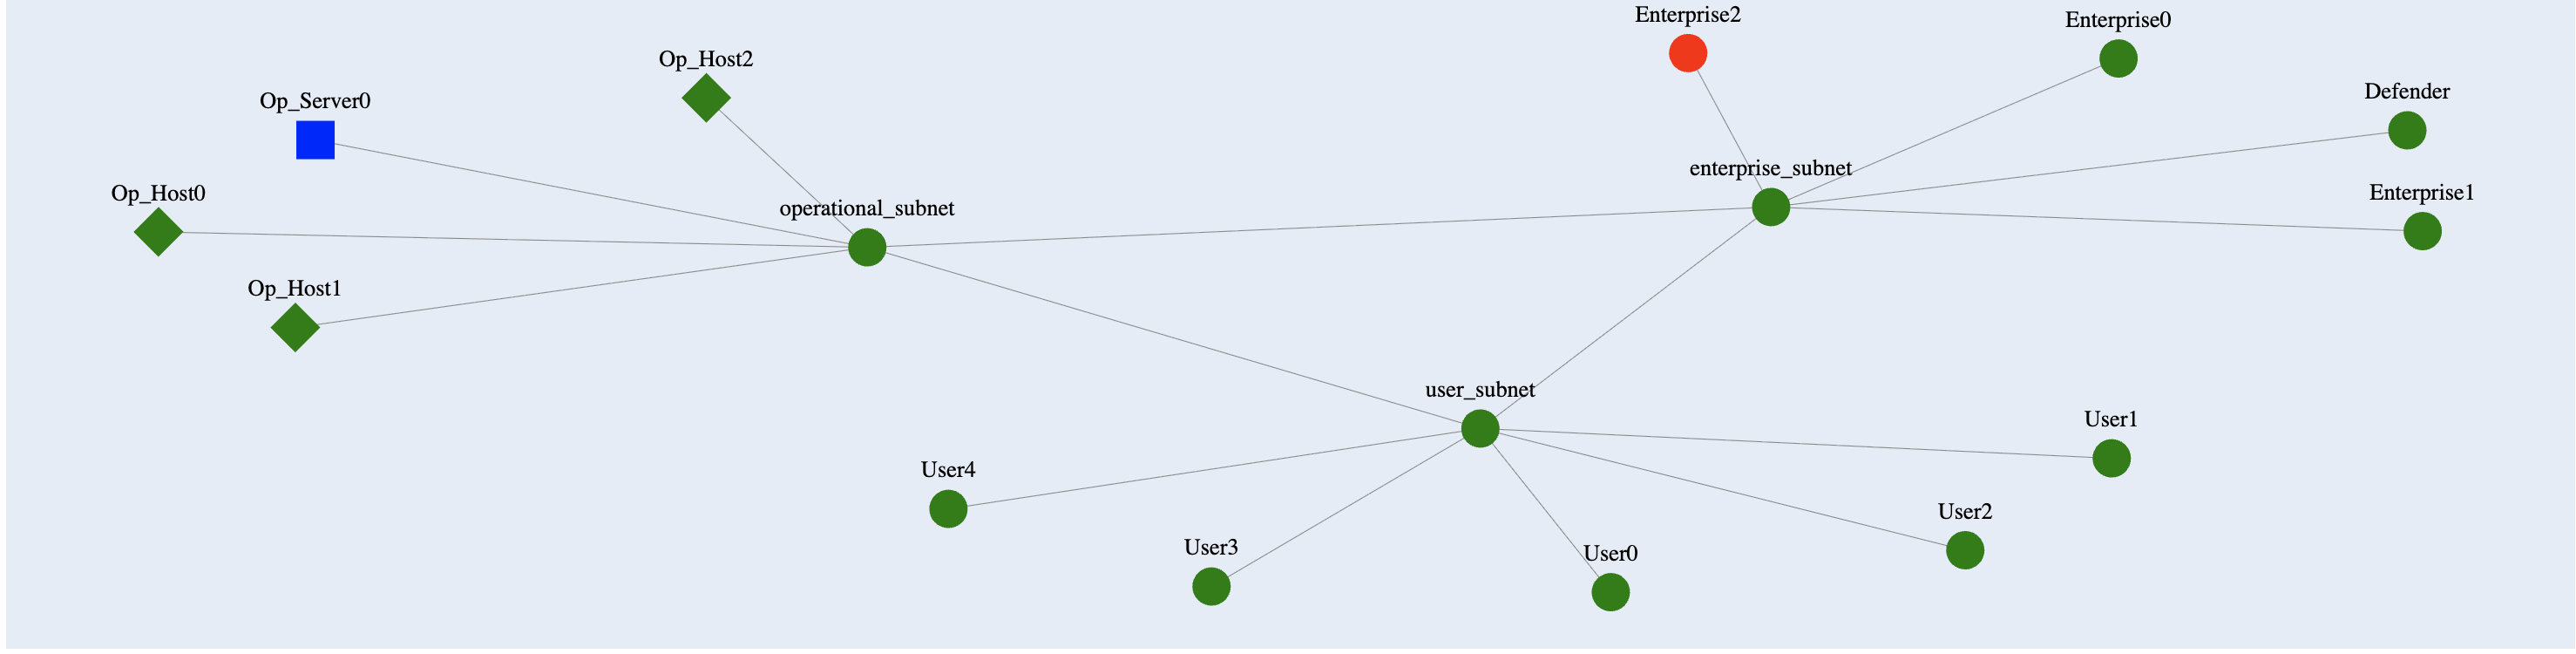
\includegraphics[width=\linewidth]{Figures/environment_state.png}
    \caption{Environment state during the attack scenario, illustrating the network topology and the red agent's activity on Enterprise2.}
    \label{fig:environment_state}
\end{figure}

Eventually, the red agent performs the action \texttt{PrivilegeEscalate\_Enterprise2} while the blue agent selects \texttt{Remove Op\_Server0}. As shown in Figure~\ref{fig:agent_action_dashboard}, this decision results in a negative step reward of $-0.1000$, indicating that the autonomous policy did not adequately mitigate the ongoing threat.

\begin{figure}[t]
    \centering
    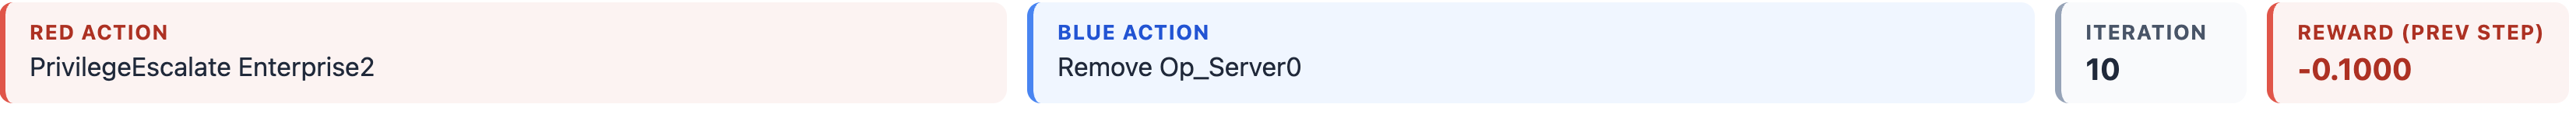
\includegraphics[width=\linewidth]{Figures/agent_action_dashboard.png}
    \caption{Dashboard view showing the red and blue actions at Iteration 10 and the resulting negative reward.}
    \label{fig:agent_action_dashboard}
\end{figure}

The dashboard highlights that the decision tree (DT) model disagrees with the RL agent's action and recommends an alternative such as \texttt{Ent0\_DecoyTomcat}, as illustrated in Figure~\ref{fig:dt_suggestion}. The SHAP-based explanation panel provides feature-level insight into why the RL policy chose (with an higher probability) the action \texttt{Remove Op\_Server0}, emphasizing inactivity-related features and prior user activity patterns.

\begin{figure}[t]
    \centering
    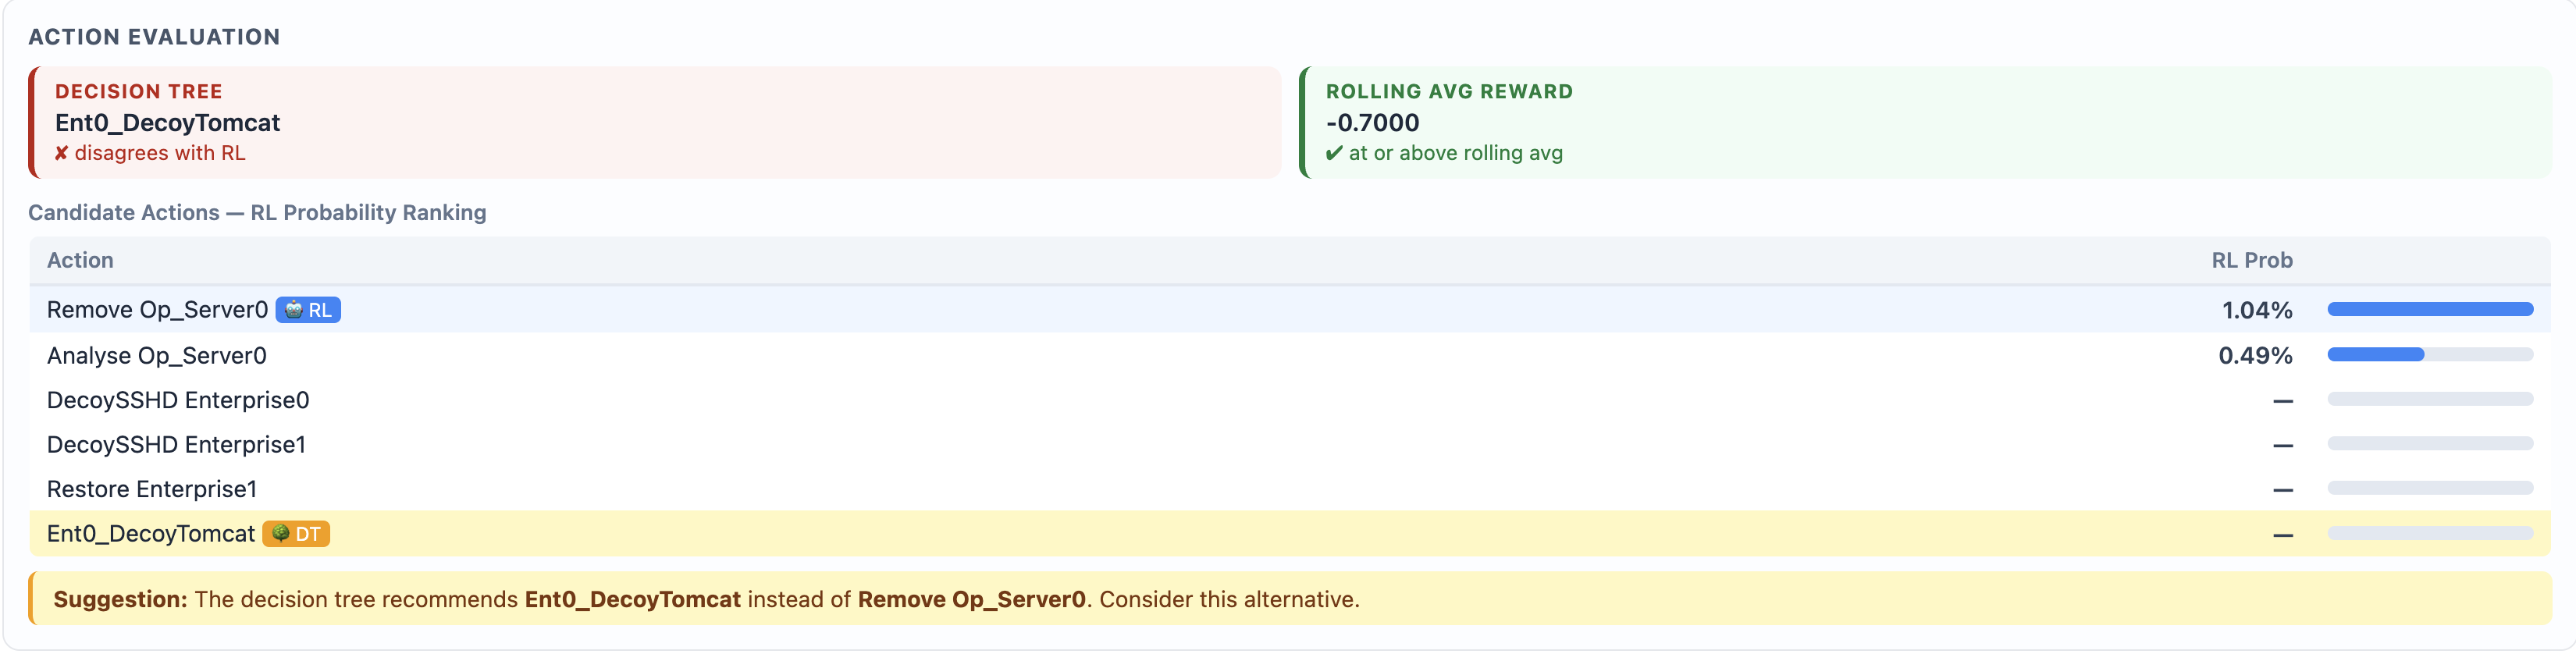
\includegraphics[width=\linewidth]{Figures/dt_suggestion.png}
    \caption{Decision tree representing the RL policy.}
    %recommendation and SHAP-based explanation highlighting feature contributions to the RL action.}
    \label{fig:dt_suggestion}
\end{figure}

However, the SHAP ranked features do not directly address the immediate adversarial activity occurring on 'Enterprise2'. The resulting negative reward demonstrates a mismatch between the learned policy's prioritization and the evolving attack context.

Next, we have a human operator observe a replay of this game, forcing the blue agent to take the same actions as before until the first human intervention. At each decision point, the operator is informed that an alternative action may be selected whenever the operator disagrees with the agent's chosen action. Figure~\ref{fig:human_override_interface} illustrates the interface that allows the operator to override the agent's action.

\begin{figure}[t]
    \centering
    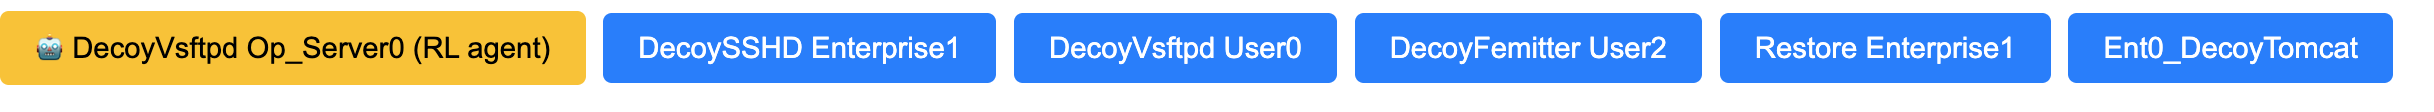
\includegraphics[width=\linewidth]{Figures/human_override_interface.png}
    \caption{Human override interface enabling intervention when the operator disagrees with the agent's selected action.}
    \label{fig:human_override_interface}
\end{figure}

When the red agent escalates privileges on 'Enterprise2', the human operator may determine, based on contextual knowledge, that the blue action should address the compromised enterprise node rather than remove an operational server.
Whenever an override occurs, the game proceeds as if the agent selected the human's alternative action, and the agent resumes selecting actions autonomously until the next intervention. This process yields a second trajectory and a reward that reflects agent performance with human intervention.

Finally, Figure~\ref{fig:dt_suggestion} conceptually illustrates the expected rewards that the human-assisted trajectory could have returned.

\begin{figure}[h]
    \centering
    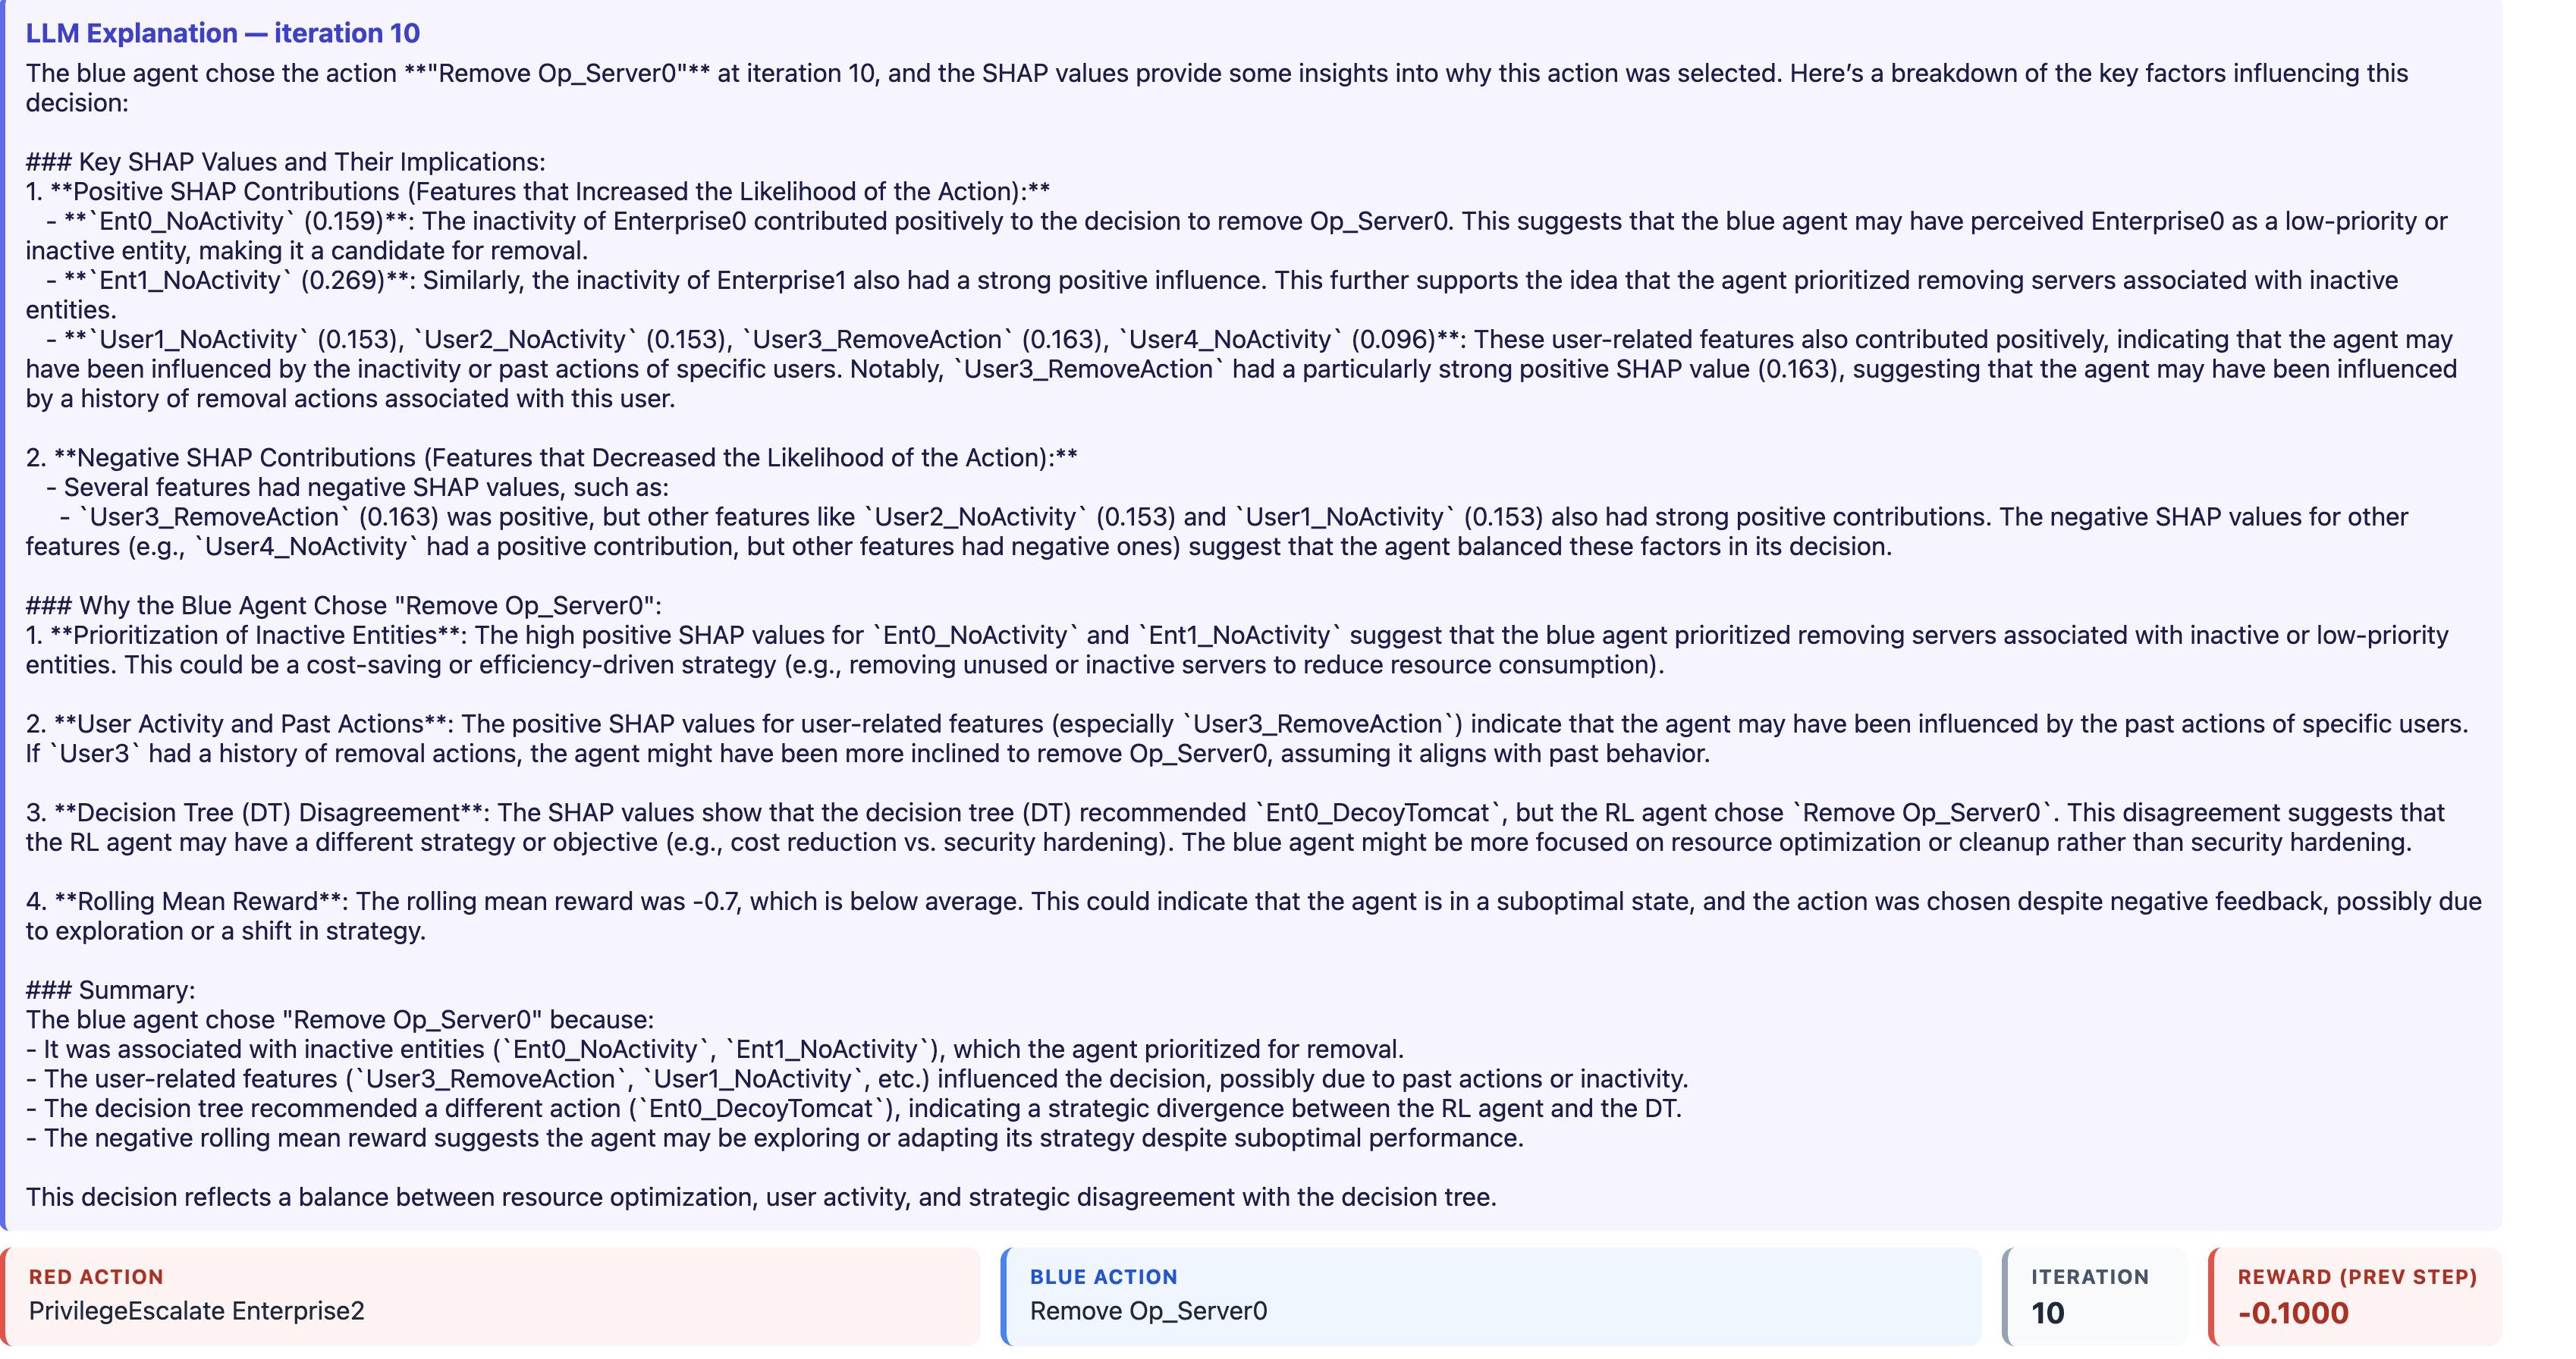
\includegraphics[width=\linewidth]{Figures/chat_log.png}
    \caption{LLM logs of human agent to determine the right action.}
    \label{fig:reward_comparison}
\end{figure}

By comparing these two rewards, we quantify the effect of human intervention on the agent's performance. In the illustrated scenario, the autonomous agent's action leads to a negative reward, whereas a human-informed alternative guided by awareness of the active attack on 'Enterprise2' better aligns with the immediate defensive objective.

The impact of human intervention is maximized when the agent's policy is suboptimal due to factors such as limited training coverage, noisy or incomplete observations, distributional shift, or modeling errors. In such cases, the Human-AI teaming framework enables strategic overrides that incorporate external domain expertise, improving overall performance as reflected by higher cumulative rewards along the intervention-enabled trajectory.

As part of our ongoing work, we are extending this framework to incorporate human actions into the training and evaluation loop to improve network resilience. We collect human intervention data during interactive cyber-defense exercises and use overrides and alternate strategies to enhance agent learning and assess their impact on system performance. By comparing agent trajectories with human interventions using metrics such as cumulative reward, recovery time, and resilience to adversarial behavior, our aim is to quantify the benefits of Human-AI teaming across scenarios and user groups.